\documentclass[conference]{IEEEtran}
\IEEEoverridecommandlockouts
% The preceding line is only needed to identify funding in the first footnote. If that is unneeded, please comment it out.
\usepackage{cite}
\usepackage[spanish]{babel}
\usepackage{amsmath,amssymb,amsfonts}
\usepackage{algorithmic}
\usepackage{graphicx}
\usepackage{textcomp}
\usepackage{xcolor}
\setlength{\parskip}{12pt}
\usepackage[numbers]{natbib}
%\renewcommand{\refname}{Referencias}
\def\BibTeX{{\rm B\kern-.05em{\sc i\kern-.025em b}\kern-.08em
    T\kern-.1667em\lower.7ex\hbox{E}\kern-.125emX}}
\begin{document}

\title{Desarrollo de sinapsis memristiva en una red neuronal pulsante implementada con transistores CMOS del nodo tecnológico SKY130\\
%{\footnotesize \textsuperscript{*}Note: Sub-titles are not captured in Xplore and should not be used}
%\thanks{Identify applicable funding agency here. If none, delete this.}
}

\author{\IEEEauthorblockN{1\textsuperscript{st} Ricardo Aldair Tirado Torres}
\IEEEauthorblockA{\textit{Centro de Investigación en Computación} \\
\textit{Instituto Politécnico Nacional}\\
Ciudad de México, México \\
rtiradot2023@cic.ipn.mx}
\and
\IEEEauthorblockN{2\textsuperscript{nd} Ricardo Barrón Fernández}
\IEEEauthorblockA{\textit{Centro de Investigación en Computación} \\
	\textit{Instituto Politécnico Nacional}\\
	Ciudad de México, México \\
	rbarron@cic.ipn.mx}
\and
\IEEEauthorblockN{3\textsuperscript{rd} Víctor Hugo Ponce Ponce}
\IEEEauthorblockA{\textit{Centro de Investigación en Computación} \\
	\textit{Instituto Politécnico Nacional}\\
	Ciudad de México, México \\
	vponce@cic.ipn.mx}
}

\maketitle

\begin{abstract}
This document is a model and instructions for \LaTeX.
This and the IEEEtran.cls file define the components of your paper [title, text, heads, etc.]. *CRITICAL: Do Not Use Symbols, Special Characters, Footnotes, 
or Math in Paper Title or Abstract.
\end{abstract}

\begin{IEEEkeywords}
Redes neuronales pulsantes, sinapsis memristiva, plasticidad dependiente del tiempo de pulso (STDP), SKY130.
\end{IEEEkeywords}

\section{Introducción}
El cómputo neuromórfico es un campo emergente en la ingeniería y la informática que se inspira en la arquitectura y funcionamiento del cerebro humano para diseñar sistemas de procesamiento de información más eficientes y adaptativos. A diferencia de las computadoras tradicionales, que siguen el modelo de von Neumann, los sistemas neuromórficos emplean una arquitectura distribuida y paralela, emulando las redes neuronales del cerebro. Esta aproximación no solo promete una mayor eficiencia energética y velocidad de procesamiento, sino también una capacidad de aprendizaje y adaptación superior.

En el corazón del cómputo neuromórfico se encuentran las redes neuronales pulsantes, que son modelos de redes neuronales que procesan información en forma de picos de actividad eléctrica, o pulsos. Estos modelos son más biológicamente realistas que las redes neuronales tradicionales utilizadas en el aprendizaje profundo. Las redes neuronales pulsantes permiten un procesamiento temporal y espacial más natural de la información, similar al que ocurre en el cerebro, lo que resulta en un rendimiento superior en tareas que requieren reconocimiento de patrones y procesamiento sensorial en tiempo real.

El aprendizaje dependiente del tiempo de los pulsos (STDP, por sus siglas en inglés) es un mecanismo clave en las redes neuronales pulsantes. El STDP es una forma de aprendizaje sináptico que ajusta la fuerza de las conexiones entre neuronas en función del momento en que ocurren los pulsos. Si una neurona emisora envía un pulso justo antes de que una neurona receptora envíe el suyo, la conexión entre ambas se fortalece. Este principio, que se observa en las sinapsis biológicas, permite a las redes neuromórficas aprender y adaptarse de manera más eficiente, logrando un aprendizaje no supervisado y dinámico. Esta regla temporal puede ser implementada directamente en unos elementos de memoria, llamados memristores, debido a su capacidad para cambiar su resistencia en función de la historia temporal de los pulsos que los atraviesan.

El memristor, un componente eléctrico cuya resistencia varía en función de la cantidad y la dirección de la carga eléctrica que lo atraviesa, ha emergido como una pieza fundamental en el campo del cómputo neuromórfico. Descubierto teóricamente por Leon Chua en 1971 y desarrollado prácticamente en los laboratorios de HP en 2008, el memristor es a menudo considerado el cuarto elemento de los circuitos pasivos junto con el resistor, el capacitor y el inductor. Su capacidad para "recordar" el último estado de resistencia hace que el memristor sea especialmente adecuado para imitar las sinapsis biológicas en sistemas neuromórficos.

En el contexto del cómputo neuromórfico, los memristores se utilizan como sinapsis artificiales que conectan las neuronas en redes neuronales pulsantes. Estas redes, que procesan información en forma de pulsos de actividad eléctrica similares a los impulsos neuronales del cerebro, se benefician enormemente de la naturaleza adaptable y no volátil del memristor. La resistencia del memristor cambia en respuesta a los picos eléctricos, permitiendo la modulación sináptica de manera analógica, lo cual es crucial para replicar los procesos de aprendizaje y memoria del cerebro humano.

Para implementar estos conceptos, se utiliza la tecnología CMOS (Complementary Metal-Oxide-Semiconductor), ampliamente conocida por su uso en la fabricación de chips de computadora tradicionales. La tecnología CMOS ofrece una plataforma robusta y escalable para desarrollar hardware neuromórfico, facilitando la creación de sistemas que son tanto energéticamente eficientes como capaces de realizar cálculos complejos en paralelo. La integración de memristores en la tecnología CMOS ha permitido avances significativos en la construcción de circuitos neuromórficos eficientes y escalables. Los memristores, debido a su tamaño reducido y bajo consumo de energía, se pueden integrar en matrices densas junto con transistores CMOS para crear chips neuromórficos que emulan el funcionamiento del cerebro humano de manera más realista y eficiente. Estos chips, como los desarrollados en proyectos como IBM TrueNorth e Intel Loihi, incorporan miles de millones de sinapsis memristivas capaces de aprendizaje autónomo y procesamiento paralelo, replicando la complejidad y eficiencia del cerebro. A medida que la tecnología CMOS sigue evolucionando, se espera que las capacidades del cómputo neuromórfico se expandan, abriendo nuevas posibilidades en la inteligencia artificial y más allá.

El cómputo neuromórfico, con sus redes neuronales pulsantes, el aprendizaje STDP y la reciente fabricación de memristores representa una revolución en cómo concebimos y desarrollamos sistemas de procesamiento de información. La integración de estos conceptos en la tecnología CMOS no solo promete un salto significativo en la eficiencia y capacidad de las máquinas, sino que también nos acerca un paso más a replicar la asombrosa complejidad y eficiencia del cerebro humano. Es por ello que, en este trabajo, se realizaron las siguientes contribuciones:

\begin{enumerate}
    \item Un circuito de neurona tipo LIF, implementada en el dominio analógico en un nivel de transistores CMOS. A través de una señal de corriente, la neurona realizará un pulso a su salida si se supera un cierto umbral y entrará en un periodo refractario.
    \item Una sinapsis del tipo memristiva, que puede cambiar su resistencia en respuesta a las señales eléctricas, lo que permite imitar la plasticidad sináptica del cerebro humano. Esta capacidad de adaptación es crucial para el aprendizaje y la memoria en sistemas neuromórficos.
    \item Una red neuronal sencilla, con una capa de entrada de x neuronas y una capa de salida de y neuronas. El nodo tecnológico empleado es el de SKY130, un proceso de fabricación de código abierto, que reduce costos asociados con el diseño y producción de chips, facilitando la creación de sistemas neuromórficos avanzados.
\end{enumerate}

\section{Sistema propuesto}

\subsection{Neurona LIF}
El circuito de una neurona LIF comprende varias secciones, como integración de corriente, fuga, generación de picos, reinicio del potencial de membrana y período refractario.

\begin{figure}[ht]
	\centering
	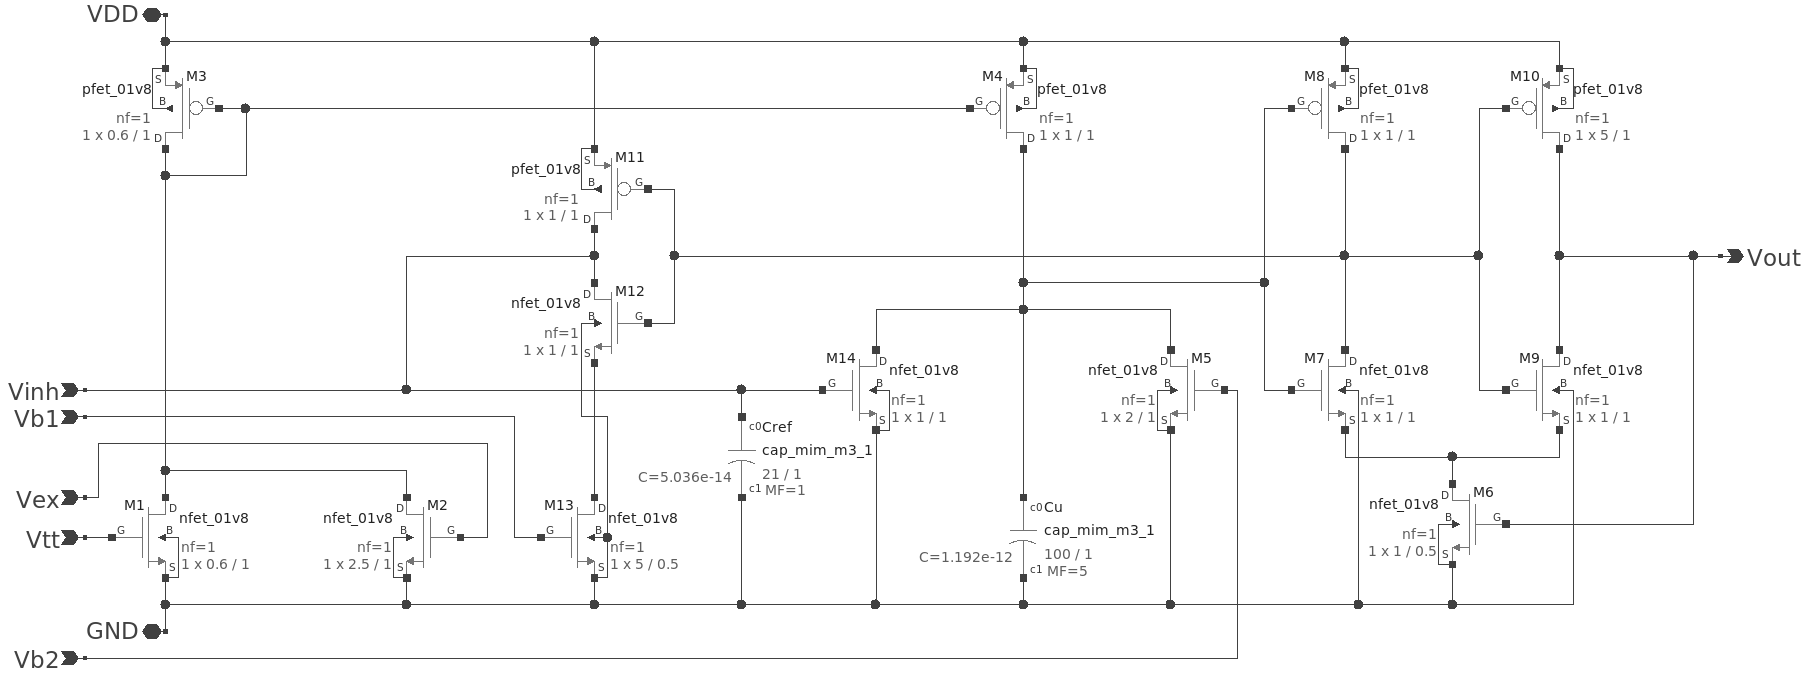
\includegraphics[scale=0.14]{img/cto_neurona_LIF.png}
	\caption{Diagrama esquemático del circuito de neurona implementado por \cite{Shamsi_2018}. Consta de varias secciones para integración de corriente, fugas, generación de picos, reinicio y período refractario.
	\label{fig:cto_neurona_LIF}}
\end{figure}

La figura \ref{fig:cto_neurona_LIF} muestra el circuito neuronal LIF propuesto originalmente, que incluye un condensador $C_{u}$ para la integración de corriente, un transistor $M_5$ para fugas, un disparador Schmitt para la generación de pulsos, $M_{11}-M_{14}$ para reinicio y un condensador $C_{ref}$ para el período refractario. Las terminales $V_{tt}$ y $V_{ex}$ se utilizan para aplicar un voltaje de entrada a la neurona, ya sea los proporcionados desde las sinapsis de retroalimentación o desde las sinapsis excitadoras laterales. La terminal inhibidora lateral $V_{inh}$ se utiliza para restablecer el potencial de membrana. Los transistores $M_{1}$ y $M_{2}$ controlan el rango de la corriente de entrada y el transistor $M_{4}$ controla la corriente inyectada en $C_{u}$. Además, la capacitancia de $C_{u}$ y $C_{ref}$ se puede alterar para controlar la tasa de pulsos de salida. Cuando se aplica el voltaje de entrada a la neurona, la corriente $I_{in}$ se inyecta en la sección del integrador con fugas a través del espejo de corriente. Luego, la corriente inyectada se integra con $C_{u}$ y se escapa a través de $M_{5}$. A través de un disparador Schmitt de baja potencia se generan los pulsos. Cuando el potencial de membrana alcanza el voltaje de conmutación del disparador Schmitt, $M_{11}-M_{14}$ intervienen para cambiar el voltaje de alto a bajo. Simultáneamente, el transistor $M_{11}$ se enciende y el potencial de membrana se restablece a cero a través de la sección de reinicio. En consecuencia, se genera un pulso en la salida de la neurona. Además, es posible restablecer el potencial de membrana a través del terminal inhibidor lateral $V_{inh}$. El circuito fue diseñado originalmente para una tecnología CMOS de 90 nm.

\begin{figure}[ht]
	\centering
	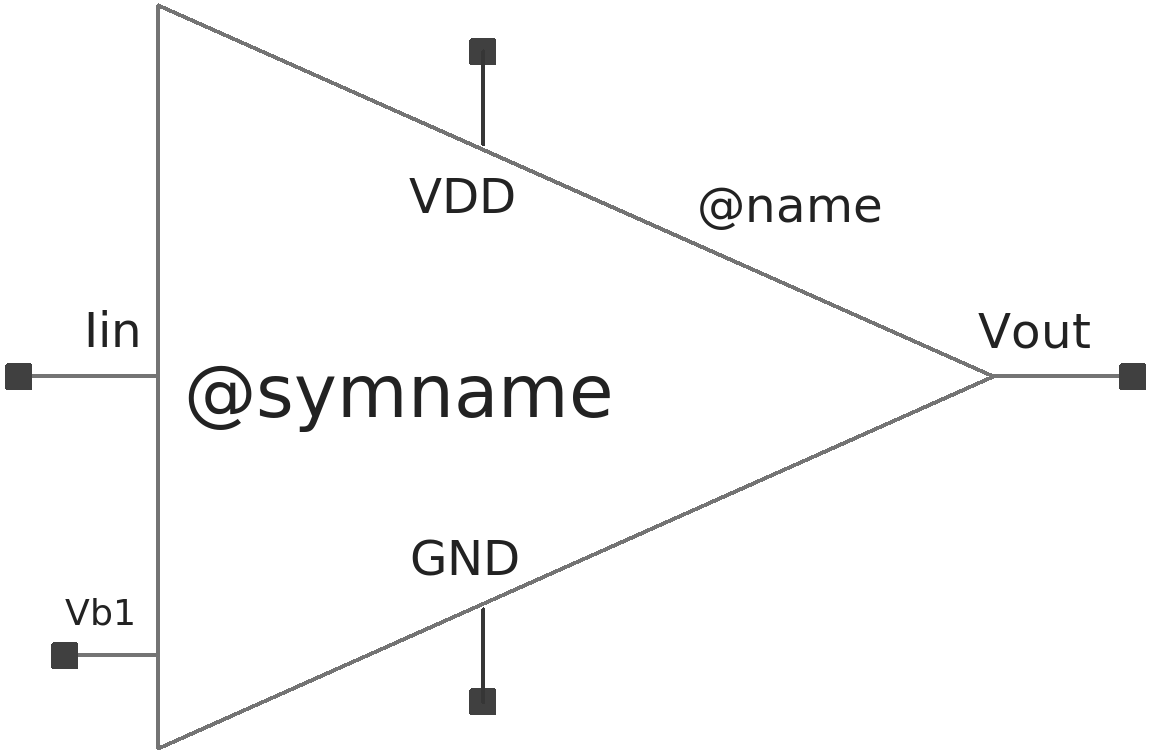
\includegraphics[scale=0.2]{img/cto_neurona_LIF_cc.png}
	\caption{Neurona LIF modificada.
		\label{fig:cto_neurona_LIF_cc}}
\end{figure}

\begin{figure}[ht]
	\centering
	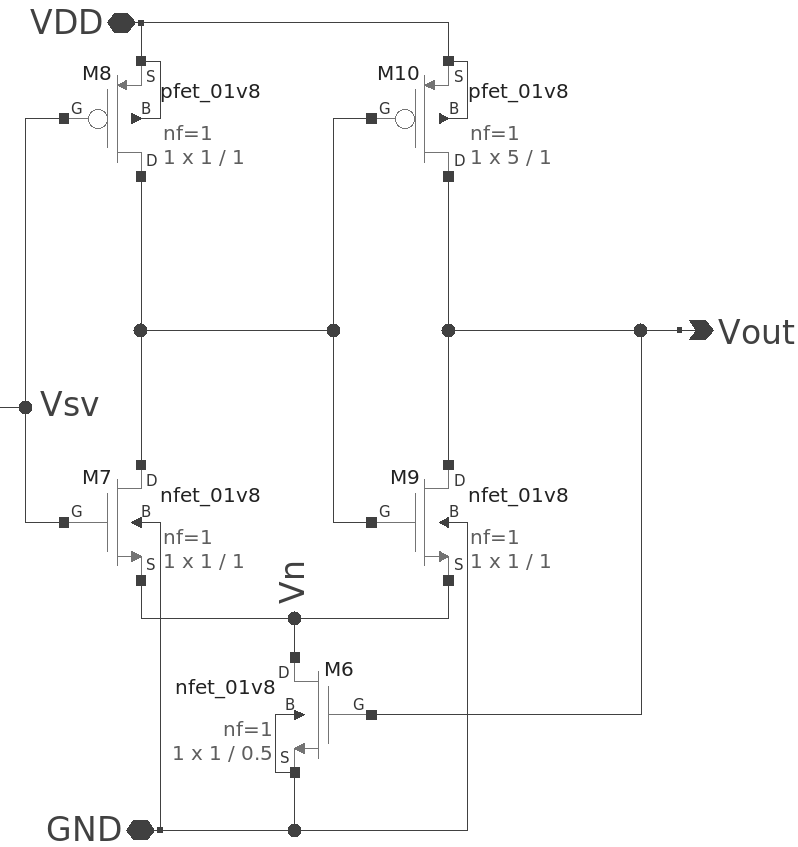
\includegraphics[scale=0.17]{img/schmitt_trigger.png}
	\caption{Diagrama esquemático de la sección correspondiente al disparador Schmitt.
		\label{fig:schmitt_trigger}}
\end{figure}

Con el objetivo de reducir el consumo de potencia, se redujo el número de transistores y se modificó la etapa de inyección del corriente del circuito, para que varié con respecto a una corriente de entrada y no a un voltaje. La implementación final, vista en la figura \ref{fig:cto_neurona_LIF_cc}, resulto en un circuito con 9 transistores (5 menos que el modelo original) y unicamente 2 entradas: La corriente de entrada a la neurona, $I_{in}$ y un voltaje de polarización $V_{b1}$, capaz de modificar la frecuencia de pulso de la neurona. De igual forma, se cambiaron los parámetros de diseño originales, para adaptar el modelo final al nodo tecnológico de SKY130, cuyo ancho de canal mínimo es de 130nm.

El funcionamiento de la neurona resulta muy parecido al original, por lo que el voltaje de conmutación, $V_{SV}$, del disparador Schmitt (Ver figura \ref{fig:schmitt_trigger}) es el umbral de activación de la neurona y se obtiene de la siguiente manera:

\begin{equation}
	I_{D6} = \beta_{6}\left(V_{n}-V_{TN}\right)^{2}
	\label{eq:ID6}
\end{equation}
\begin{equation}
	I_{D7} = \beta_{7}\left(V_{DD}-V_{SV}-V_{TP}\right)^{2}
	\label{eq:ID7}
\end{equation}
\begin{equation}
	I_{D8} = \beta_{8}\left(V_{SV}-V_{n}-V_{TN}\right)^{2}
	\label{eq:ID8}
\end{equation}

En donde $V_{TN}$ y $V_{TP}$ son los voltajes de umbral de los transistores de canal N y P, respectivamente y $\beta_{N}$ es el parámetro de transconductancia que equivale a $\mu C_{OX} \frac{W}{L}$. Igualando la ecuación \ref{eq:ID7} y \ref{eq:ID8} para despejar a $V_{SV}$, se obtiene:

\begin{equation}
	V_{SV} = \frac{R_{7/8}(V_{DD}-V_{TP})+V_{n}+V_{TN}}{R_{7/8}+1}
	\label{eq:VSV1}
\end{equation}

En donde $R_{7/8}$ representa a $\sqrt{\frac{\beta_{7}}{\beta_{8}}}$. Igualando la ecuación \ref{eq:ID6} y \ref{eq:ID8} para despejar a $V_{n}$, se obtiene:

\begin{equation}
	V_{n} = \frac{V_{SV}+(R_{6/8}-1)V_{TN}}{R_{6/8}+1}
	\label{eq:Vn}
\end{equation}

En donde $R_{6/8}$ representa a $\sqrt{\frac{\beta_{6}}{\beta_{8}}}$. Sustituyendo la ecuación \ref{eq:Vn} en \ref{eq:VSV1}, se obtiene:

\begin{equation}
	V_{SV} = \frac{R_{7/8}(V_{DD}-V_{TP})+\left(\frac{R_{6/8}-1}{R_{6/8}+1}+1\right)V_{TN}}{\left(R_{7/8}+1\right)-\frac{1}{R_{6/8}+1}}
	\label{eq:VSV2}
\end{equation}

\subsection{Sinapsis memristiva}
La configuración 6T1R, empleada en la sinapsis memristiva, fue tomada en base a la idea planteada en \cite{Tian_2022}, donde se implementan 4 transistores en configuración de puente H para controlar el sentido de la corriente que pasa por un memristor. El modelo de simulación pertenece a la tecnología SKY130 de \cite{SKY130reram}\cite{SKY130reramGitHub}, pero los parámetros del dispositivo son los tomados por \cite{Wang_2016}\cite{Alshaya_2022}. Este memristor tiene 

El modelo básico de la regla STDP esta determinado por la ecuación \ref{eq:STDP}:

\begin{equation}
    \quad \Delta w
        \left \{
            \begin{aligned}
                A^{+}e^{-\Delta t/\tau^{+}}, & & \text{si} & & \Delta t > 0 \\
                -A^{-}e^{\Delta t/\tau^{-}}, & & \text{si} & & \Delta t < 0
            \end{aligned}
        \right.
    \label{eq:STDP}
\end{equation}

Ahora bien, para que el exista una potenciación

\section{Operación del sistema}

\section{Resultados de la simulación}


\subsection{Figures and Tables}
\paragraph{Positioning Figures and Tables} Place figures and tables at the top and 
bottom of columns. Avoid placing them in the middle of columns. Large 
figures and tables may span across both columns. Figure captions should be 
below the figures; table heads should appear above the tables. Insert 
figures and tables after they are cited in the text. Use the abbreviation 
``Fig.~\ref{fig}'', even at the beginning of a sentence.

\begin{table}[htbp]
\caption{Parámetros $\frac{W}{L}$ de la neurona LIF}
\begin{center}
\begin{tabular}{|c|c|c|c|}
\hline
\textbf{Table}&\multicolumn{3}{|c|}{\textbf{Table Column Head}} \\
\cline{2-4} 
\textbf{Head} & \textbf{\textit{Table column subhead}}& \textbf{\textit{Subhead}}& \textbf{\textit{Subhead}} \\
\hline
copy& More table copy$^{\mathrm{a}}$& &  \\
\hline
\multicolumn{4}{l}{$^{\mathrm{a}}$Sample of a Table footnote.}
\end{tabular}
\label{tab1}
\end{center}
\end{table}

\begin{table}[htbp]
\caption{Parámetros $\frac{W}{L}$ de la sinapsis memristiva}
\begin{center}
\begin{tabular}{|c|c|c|c|}
\hline
\textbf{Table}&\multicolumn{3}{|c|}{\textbf{Table Column Head}} \\
\cline{2-4} 
\textbf{Head} & \textbf{\textit{Table column subhead}}& \textbf{\textit{Subhead}}& \textbf{\textit{Subhead}} \\
\hline
copy& More table copy$^{\mathrm{a}}$& &  \\
\hline
\multicolumn{4}{l}{$^{\mathrm{a}}$Sample of a Table footnote.}
\end{tabular}
\label{tab1}
\end{center}
\end{table}

\begin{figure}[htbp]
\centerline{
\includegraphics{img/fig1.png}}
\caption{Example of a figure caption.}
\label{fig}
\end{figure}

\section*{Conclusión}

Este trabajo presento una implementación de neuronas LIF interconectadas entre sí, a través de un modelo de sinapsis 6T1R, cuyo componente principal era el memristor, el cual proporcionó diferentes pesos sinápticos de acuerdo con la regla de aprendizaje STDP. La construcción del sistema se hizo por medio de la herramienta de diseño esquemático Xschem y la simulación con NGSPICE. Cabe señalar que se utilizó la tecnología de SKY130, desarrollado por SkyWater Technology en colaboración con Google, que es un proceso de fabricación de semiconductores que ha sido puesto a disposición de la comunidad de diseño de circuitos de manera abierta y gratuita. Esto facilita la innovación y reduce significativamente los costos asociados con el diseño y la producción de chips, haciendo más accesible la experimentación y el desarrollo de nuevas tecnologías. Dentro de los elementos proporcionados por este nodo tecnológico, se encuentra el memristor, una tecnología clave que facilita la implementación de sinapsis artificiales en sistemas neuromórficos, soportando redes neuronales pulsantes y el aprendizaje STDP. Su capacidad para cambiar de estado de manera no volátil y su integración en la tecnología CMOS permiten la creación de sistemas de cómputo avanzados que no solo son más eficientes energéticamente, sino también más apto de emular las capacidades adaptativas y de aprendizaje del cerebro humano. La convergencia de estas tecnologías promete revolucionar el campo de la inteligencia artificial, llevando el rendimiento y la eficiencia del cómputo a nuevos niveles.

\bibliographystyle{IEEEtranN}
\bibliography{ref/referencias.bib}

\end{document}
